\documentclass[aspectratio=169]{beamer}
\usepackage{basileabeam}

% Notes:
%\pgfpagesuselayout{2 on 1}[a4paper,border shrink=5mm]
%\setbeamertemplate{note page}[plain]
%\setbeameroption{show notes on second screen=bottom}

\title              {Cuteserver}

\author             {Rahel Kempf, Ephraim Siegfried}
\institute          {Operating Systems, University of Basel}

\date               {14.06.2024}

\ulogo        		{Template/header}
\ulistelement    	{Template/listelement}

\graphicspath{{Figures/}}

% Options:
\totalNoSlidesDisabled % To turn off the total number of slides in the footer. Comment this if you want the total number of slides in the footer

\headerSectionsDisabled % Comment this if you want a fancy header containing your sections.


\begin{document}

\begin{frame}[t,plain]
\titlepage
\end{frame}

\note{Notes can help you to remember important information. Turn on the notes option.}
\begin{frame}[c]{Problem Statement}
\begin{columns}[c]
    \column{.55\textwidth}
        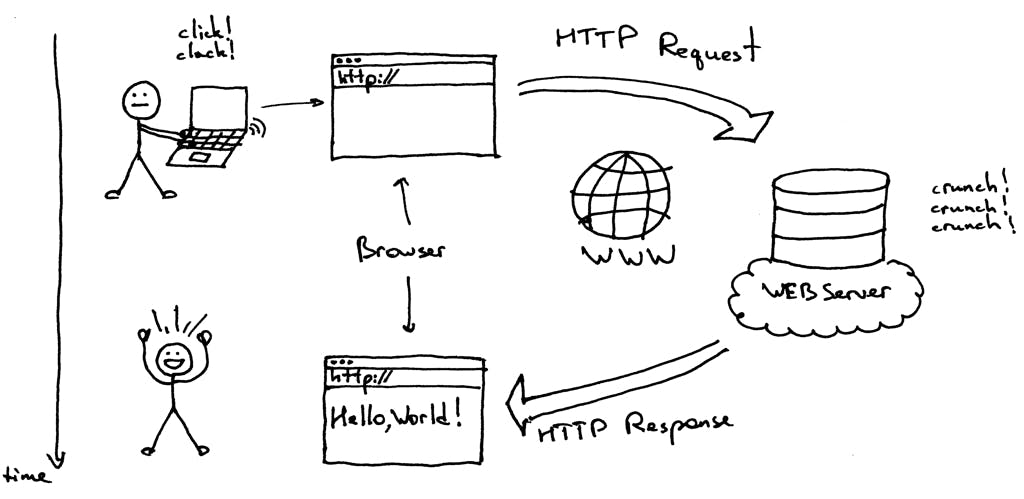
\includegraphics[width=\textwidth,height=\textheight,keepaspectratio]{webserver-comic.jpg}
    \column{.45\textwidth}
   We visit web pages all the time and want to understand the underlying processes. Therefore we want to build our own web server.
\end{columns}
\end{frame}

\begin{frame}[c]{Features}
   \begin{itemize}
       \item Multiple Users can connect concurrently 
       \item Error handling 
   \end{itemize} 
\end{frame}

\begin{frame}[c]{Progress Pictues}
  \centering
  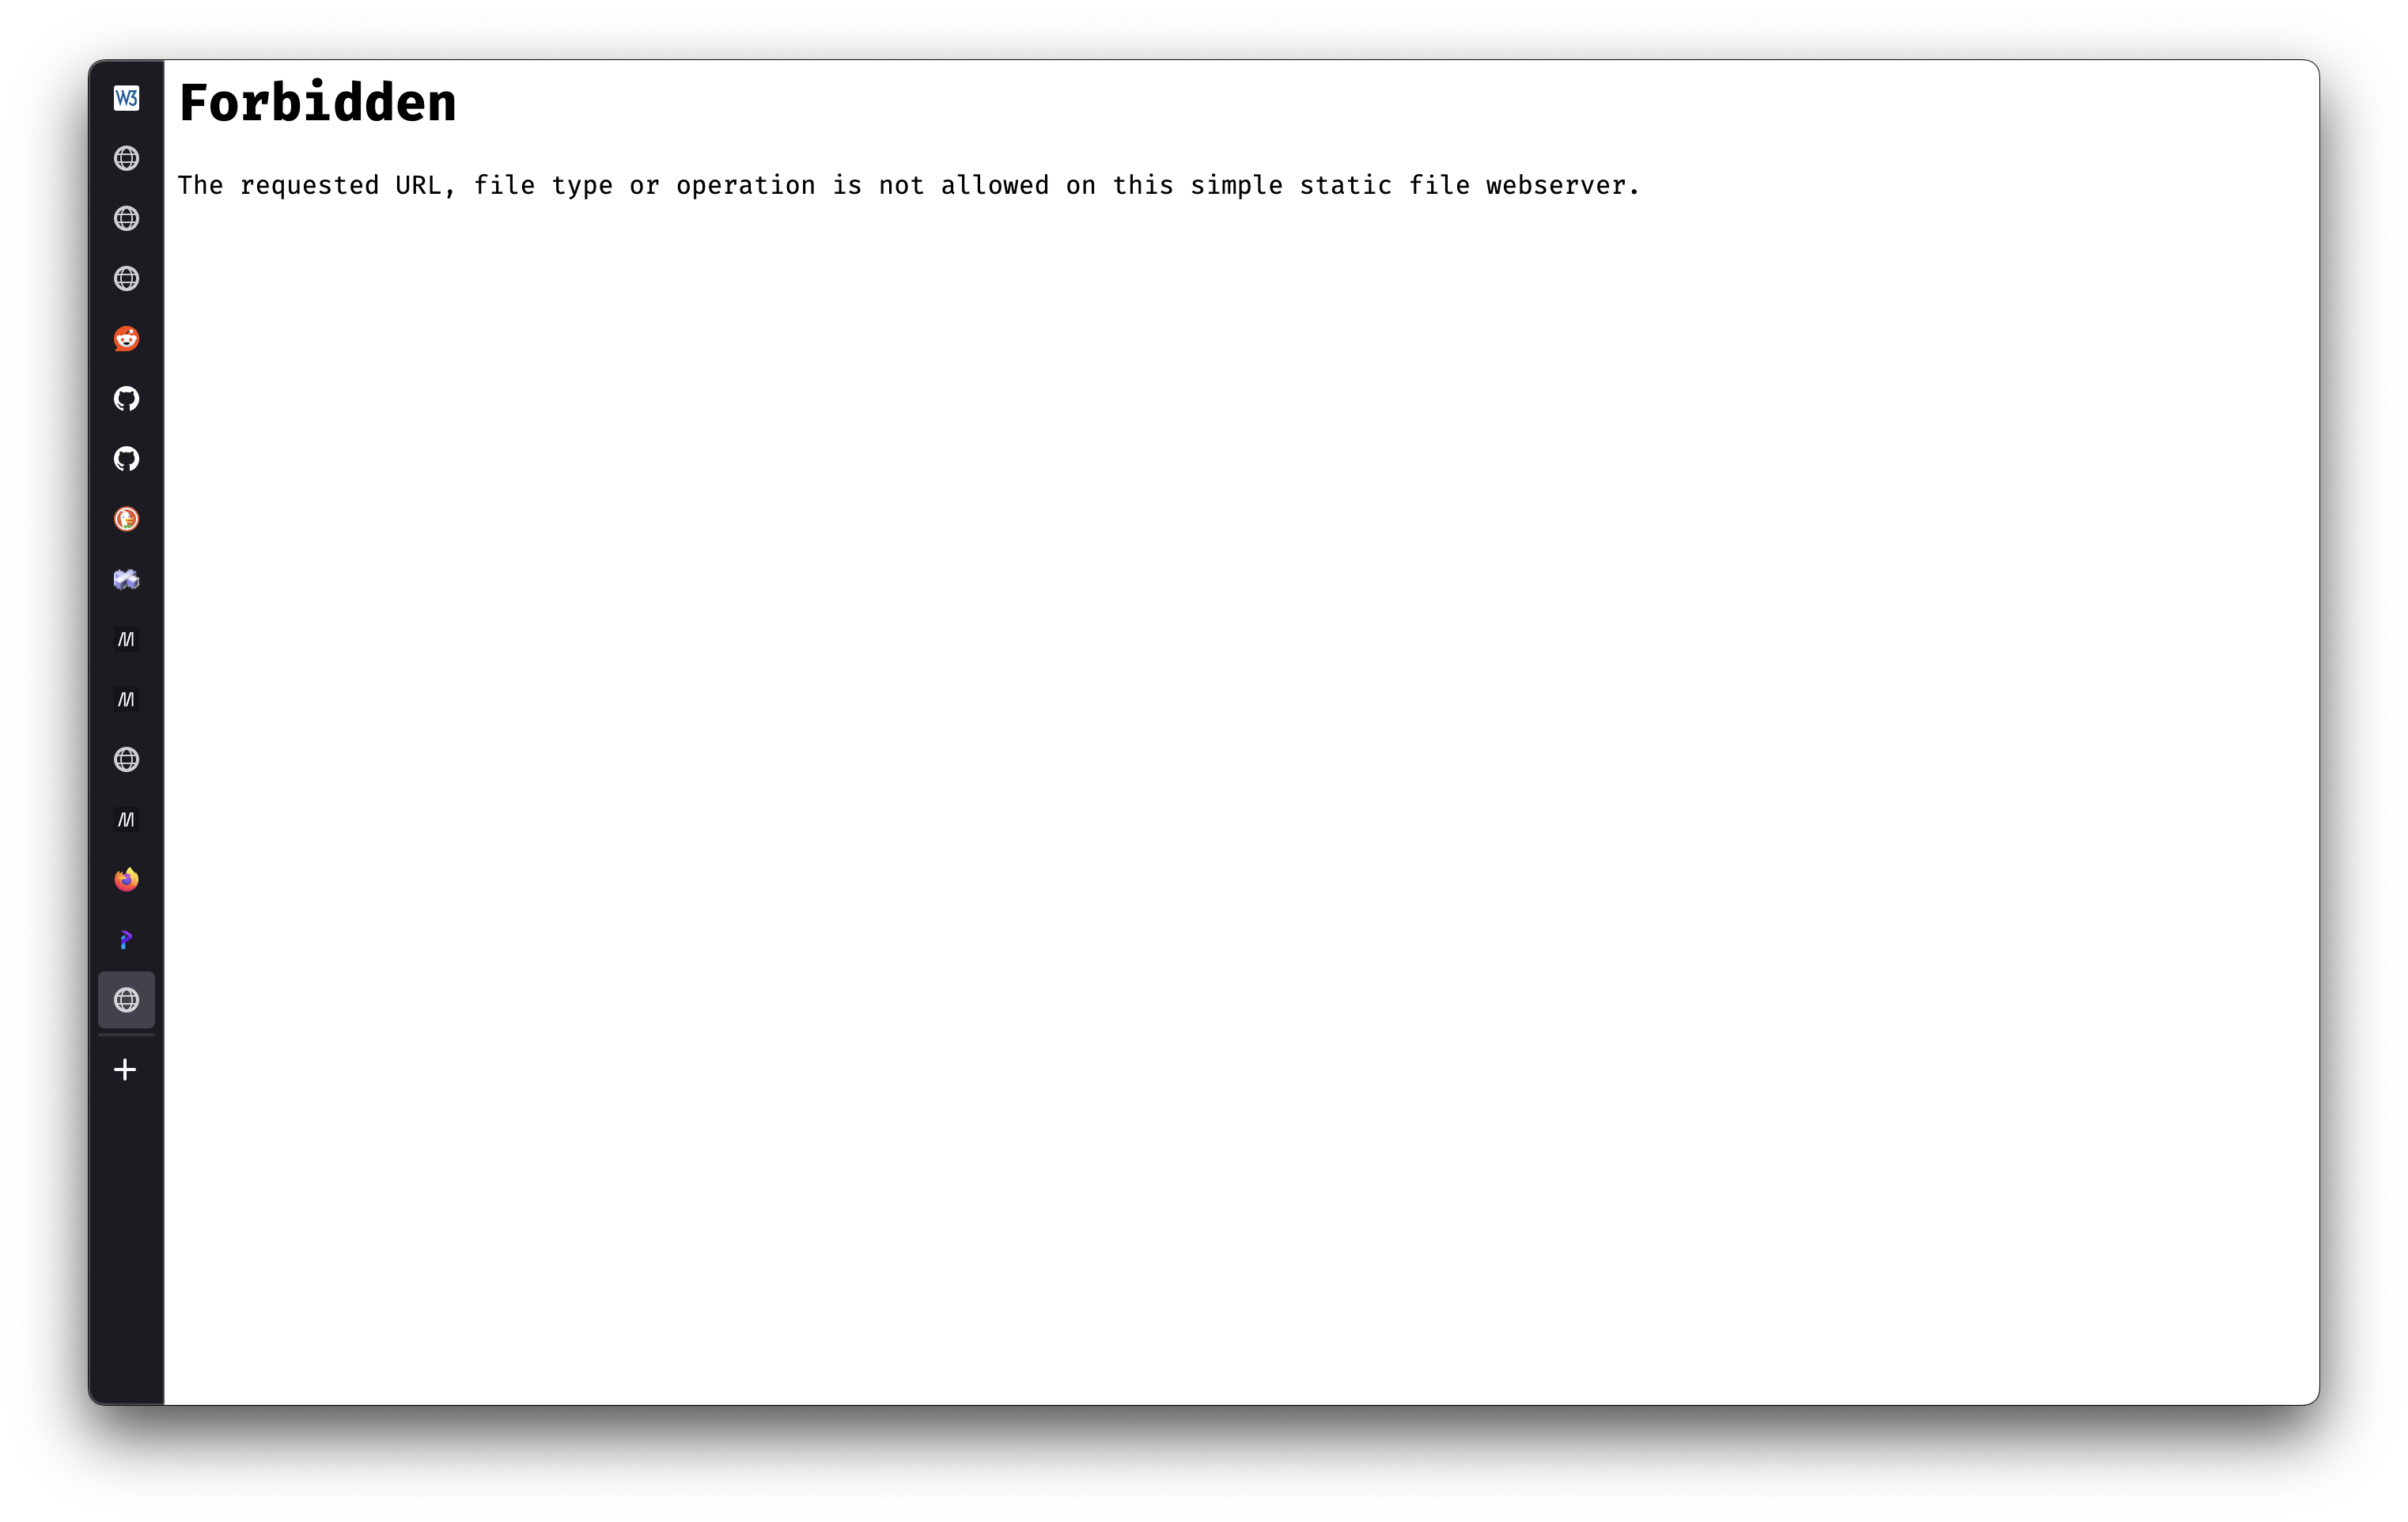
\includegraphics[width=0.8\textwidth,height=\textheight,keepaspectratio]{00_errors.png}
\end{frame}

\begin{frame}[c]{}
  \centering
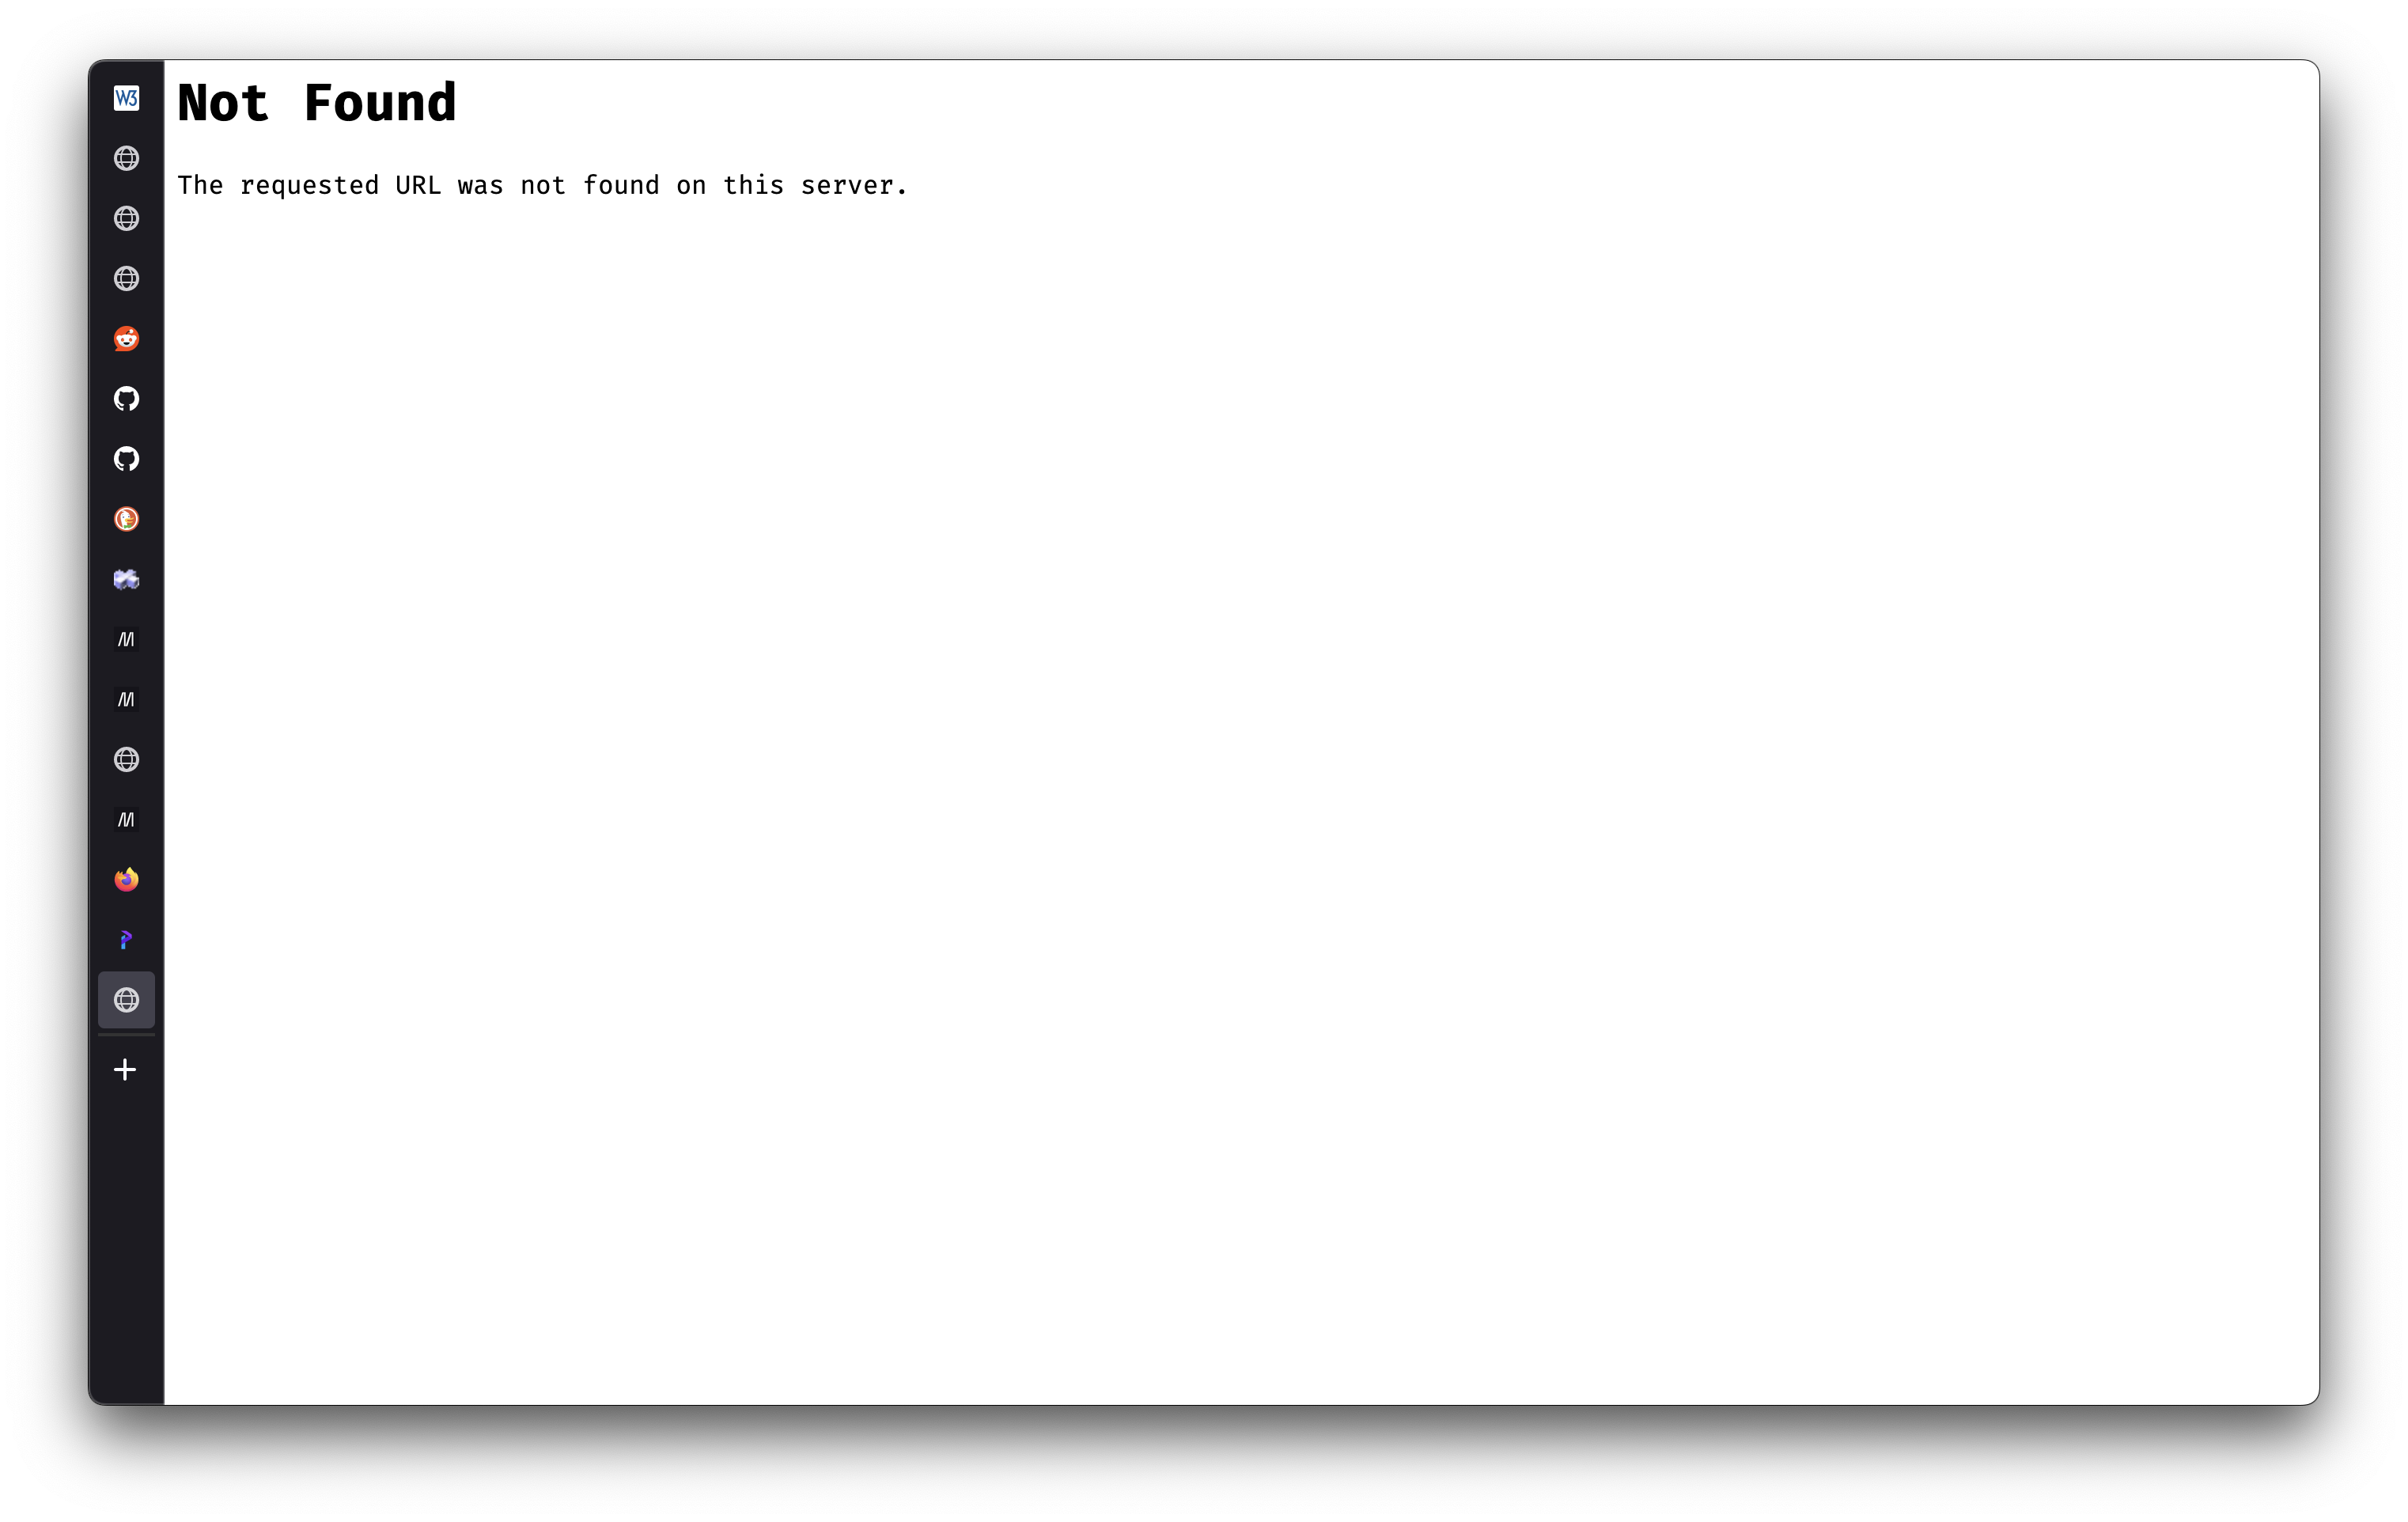
\includegraphics[width=0.8\textwidth,height=\textheight,keepaspectratio]{00_errors1.png}
\end{frame}

\begin{frame}[c]{}
  \centering
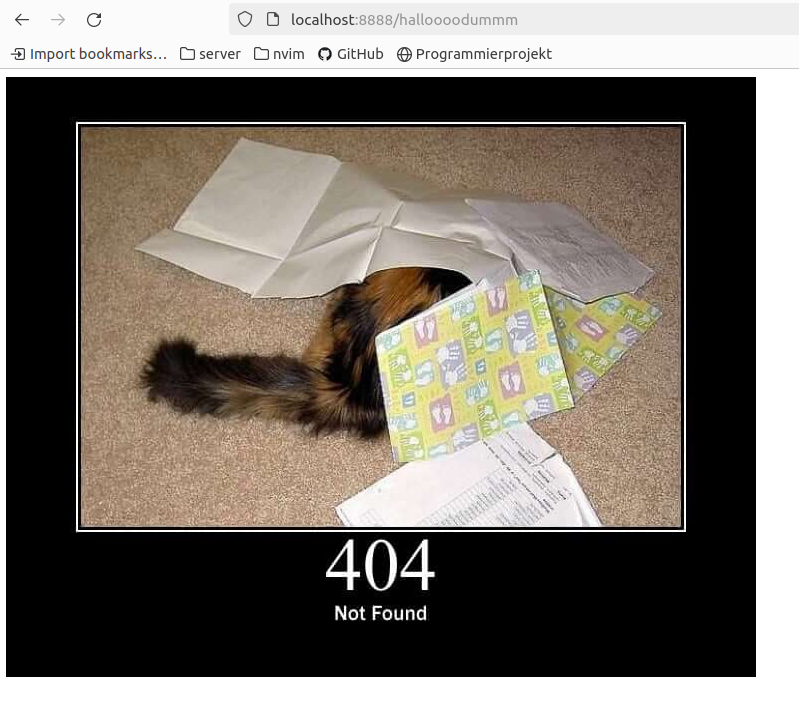
\includegraphics[width=0.8\textwidth,height=\textheight,keepaspectratio]{02_http_cats.png}
\end{frame}

\begin{frame}[c]{Features}
    \begin{columns}[c]
        \column{.55\textwidth}
           \begin{itemize}
               \item Multiple Users can connect concurrently 
               \item Error handling 
               \item Process HTTP Requests (GET, POST, HEAD)
           \end{itemize} 
        \column{.45\textwidth}
            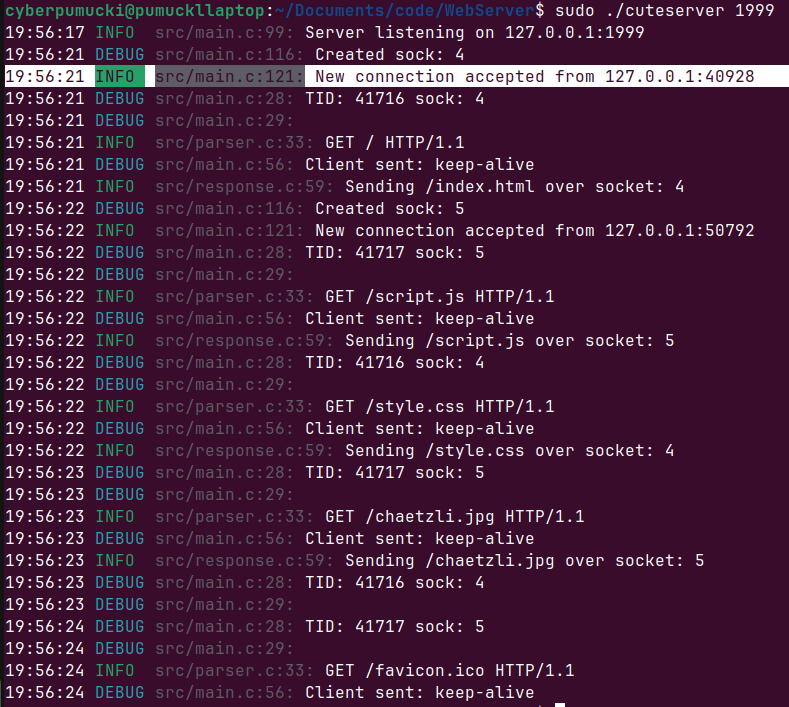
\includegraphics[width=\textwidth,height=\textheight,keepaspectratio]{keep-alive.png}
    \end{columns}
\end{frame}

\begin{frame}[c]{}
  \centering
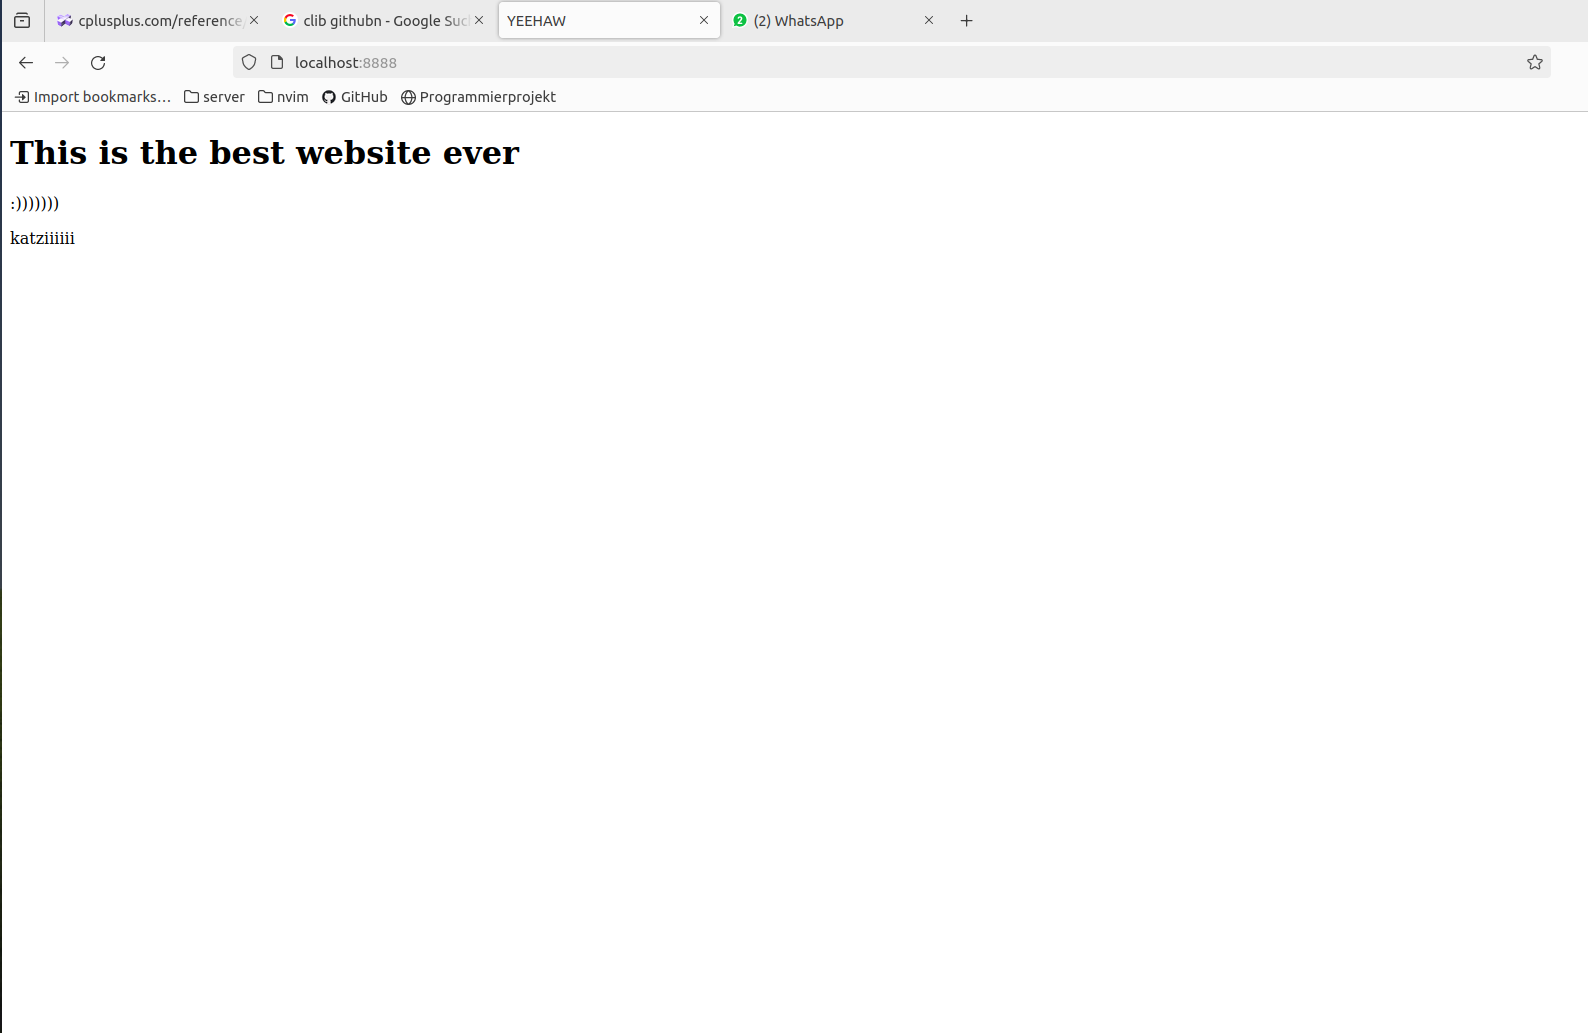
\includegraphics[width=0.8\textwidth,height=\textheight,keepaspectratio]{01_bare_html.png}
\end{frame}

\begin{frame}[c]{}
  \centering
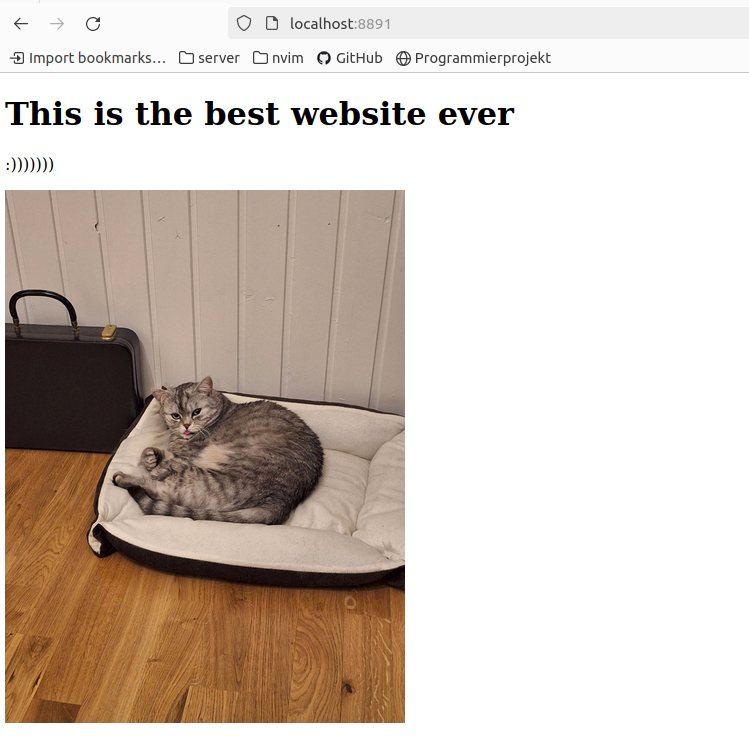
\includegraphics[width=0.8\textwidth,height=\textheight,keepaspectratio]{03_html_mit_bild.png}
\end{frame}

\begin{frame}[c]{}
  \centering
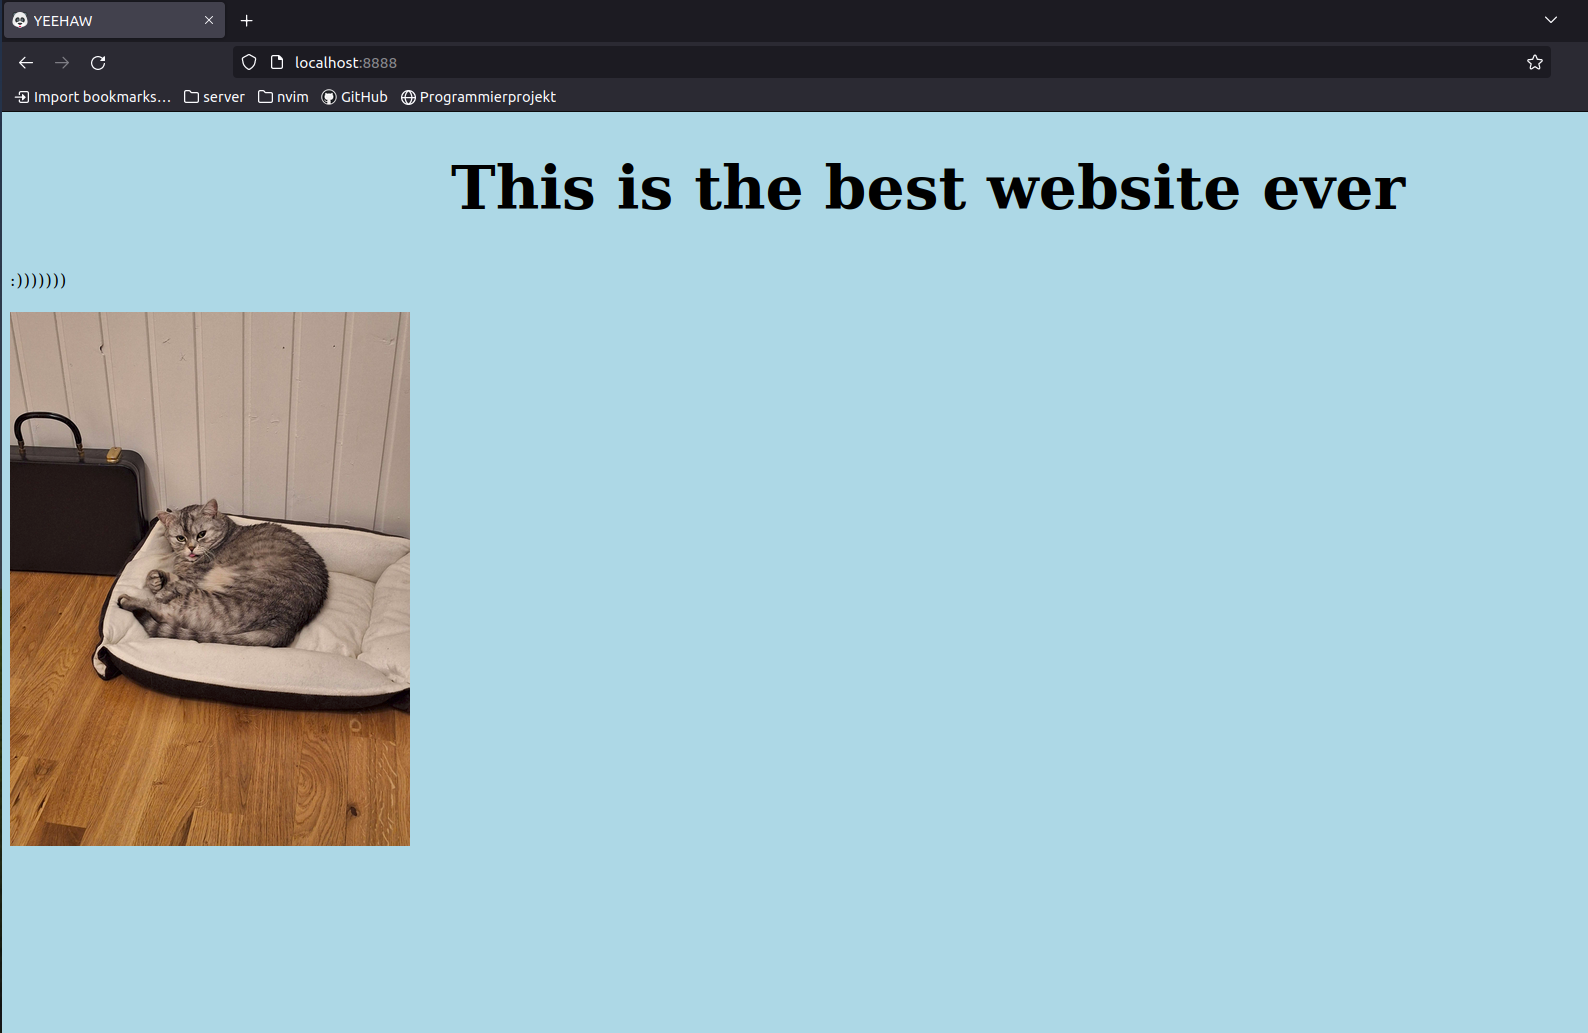
\includegraphics[width=0.8\textwidth,height=\textheight,keepaspectratio]{04_somecss.png}
\end{frame}

\begin{frame}[c]{Features}
   \begin{itemize}
       \item Multiple Users can connect concurrently 
       \item Error handling 
       \item Process HTTP Requests (GET, POST, HEAD)
       \item CGI (Common Gateway Interface) Support
   \end{itemize} 
\end{frame}

\begin{frame}[c]{}
  \centering
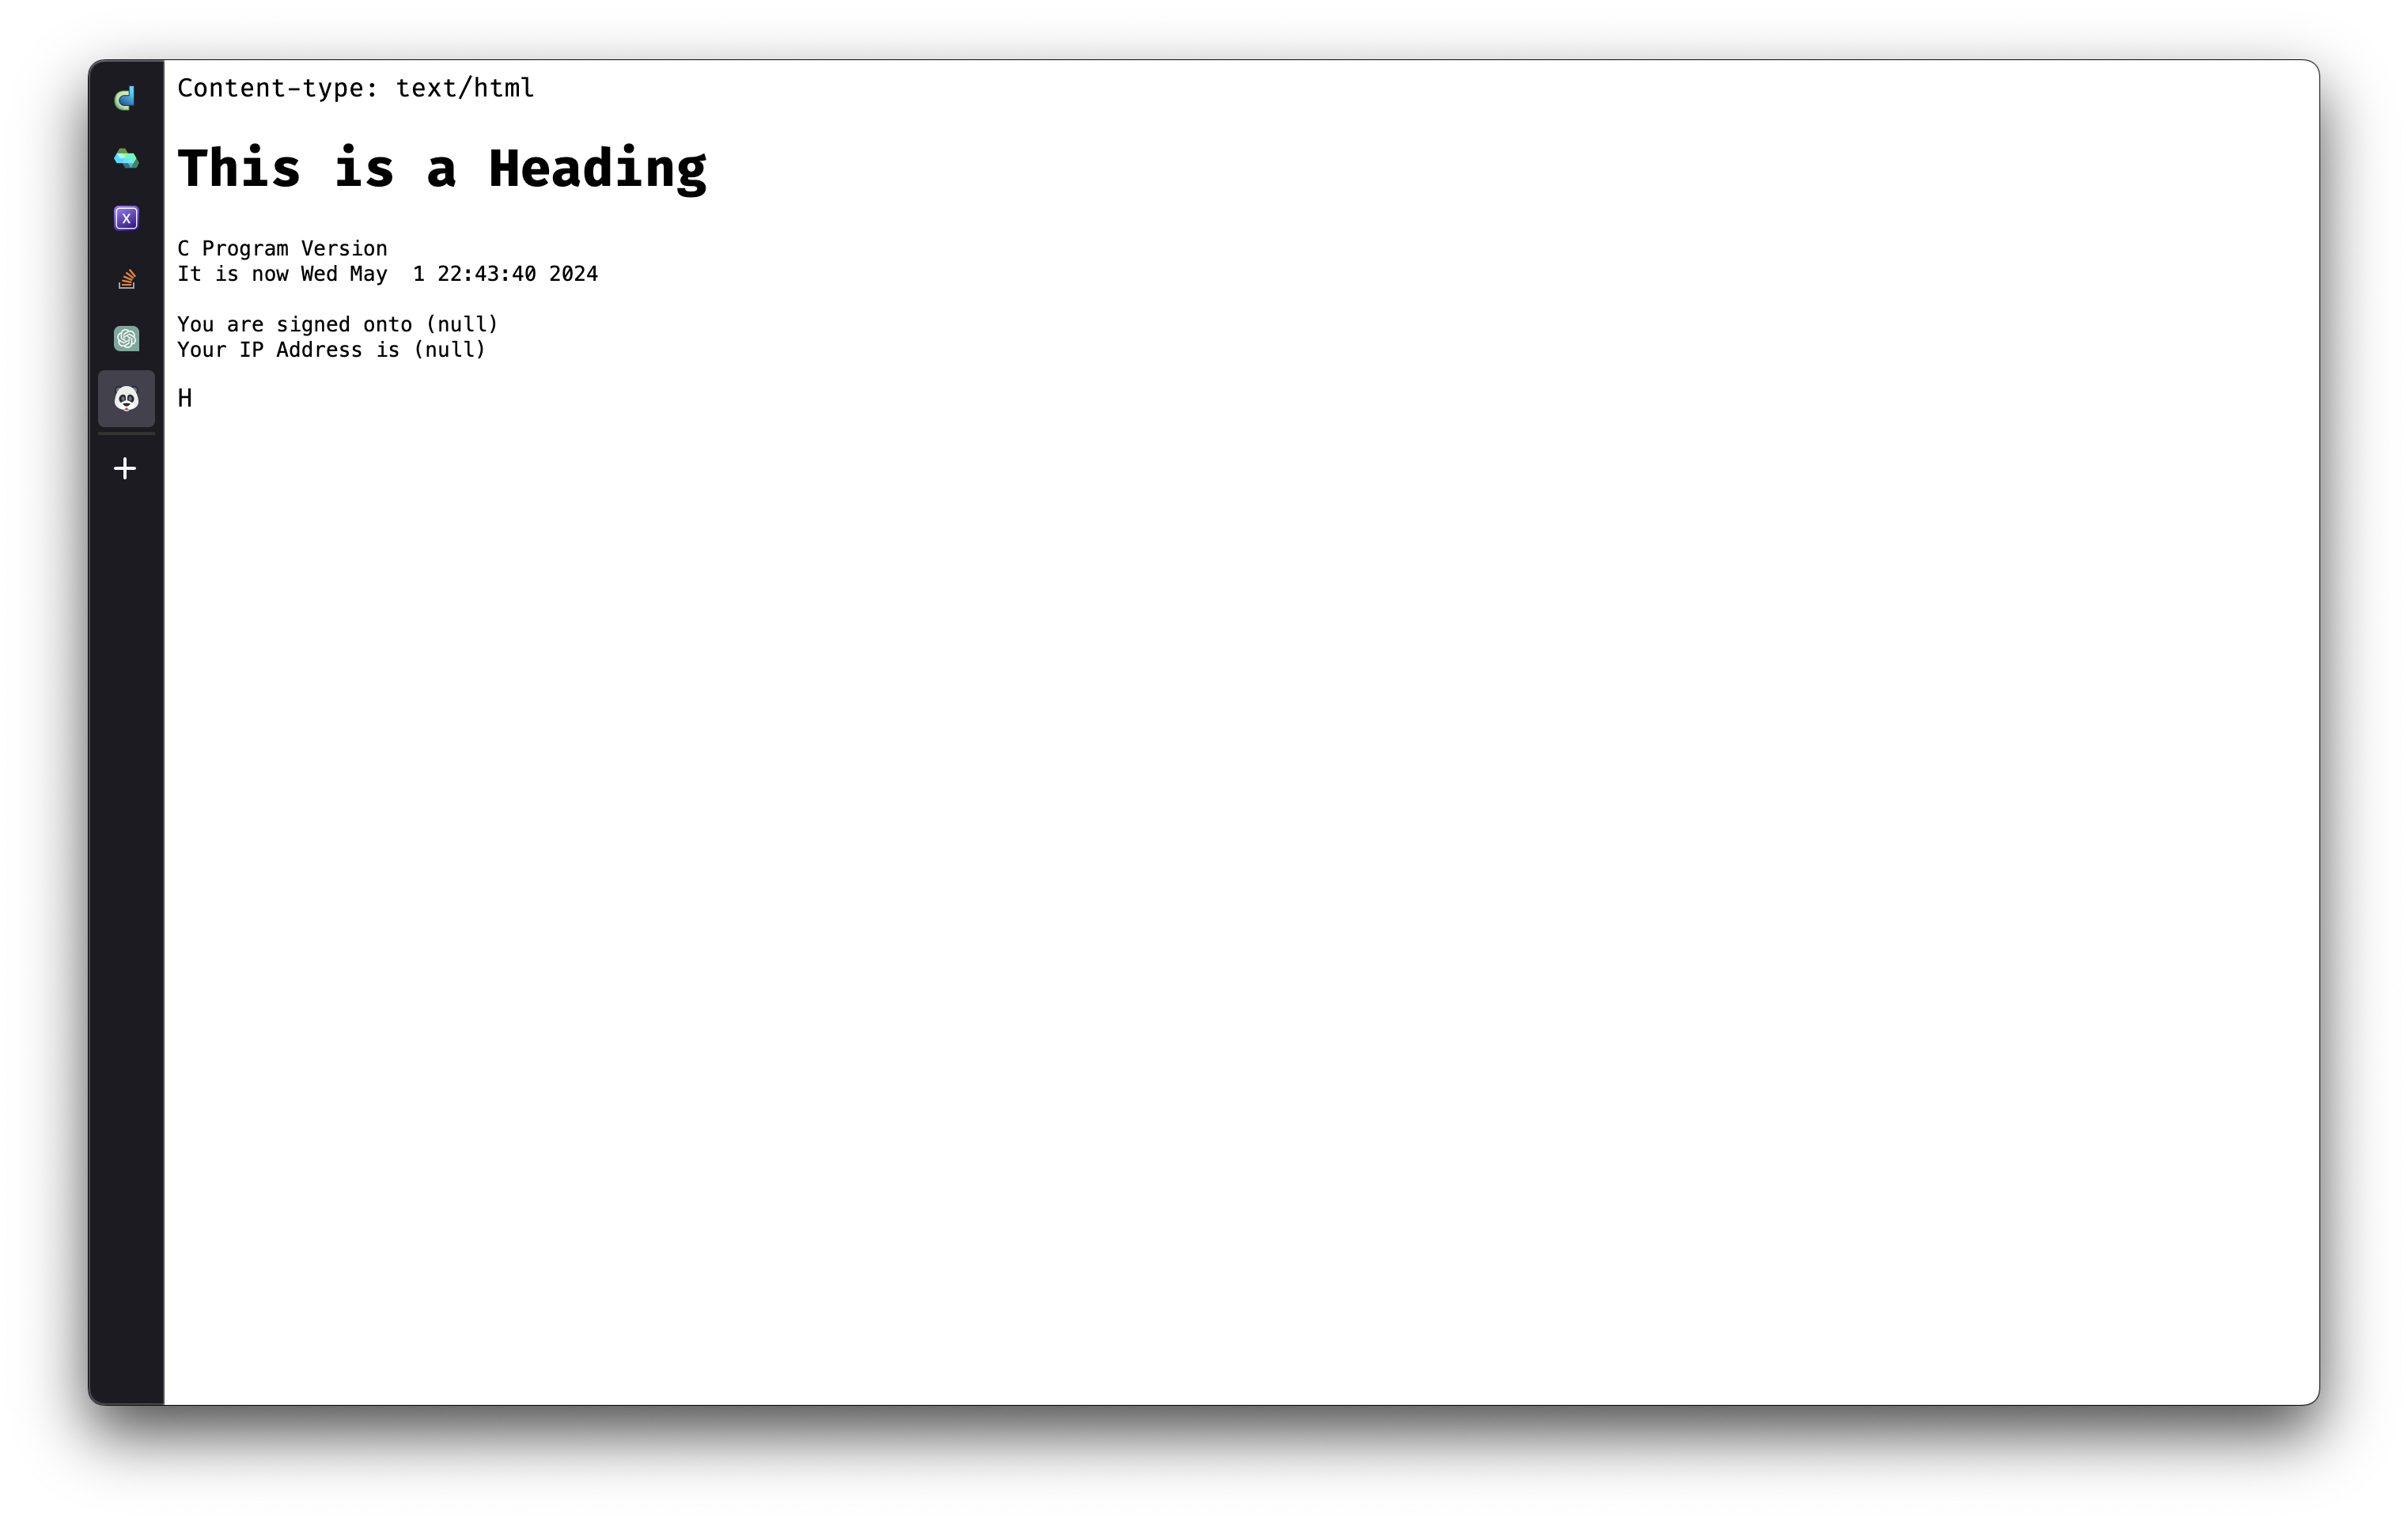
\includegraphics[width=0.8\textwidth,height=\textheight,keepaspectratio]{05_firstCGI.png} 
\end{frame}

\begin{frame}[c]{}
  \centering
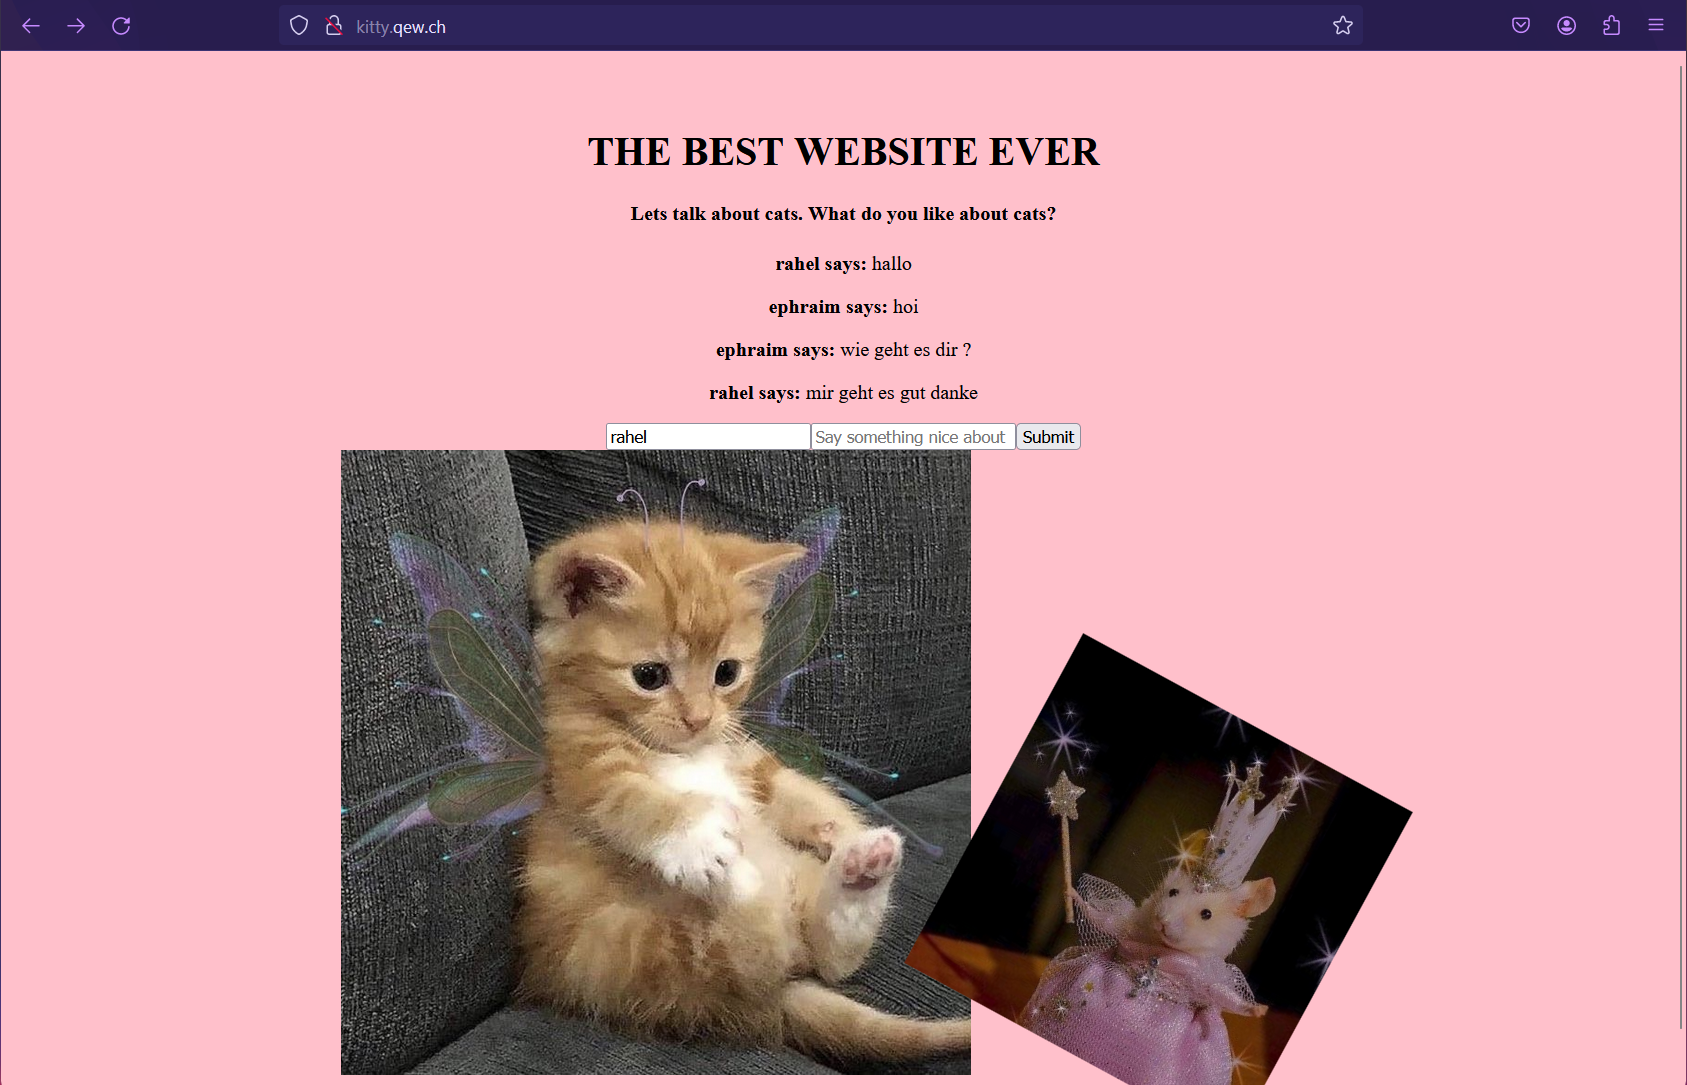
\includegraphics[width=0.8\textwidth,height=\textheight,keepaspectratio]{06_ephi_app.png}
\end{frame}

\begin{frame}[c]{}
  \centering
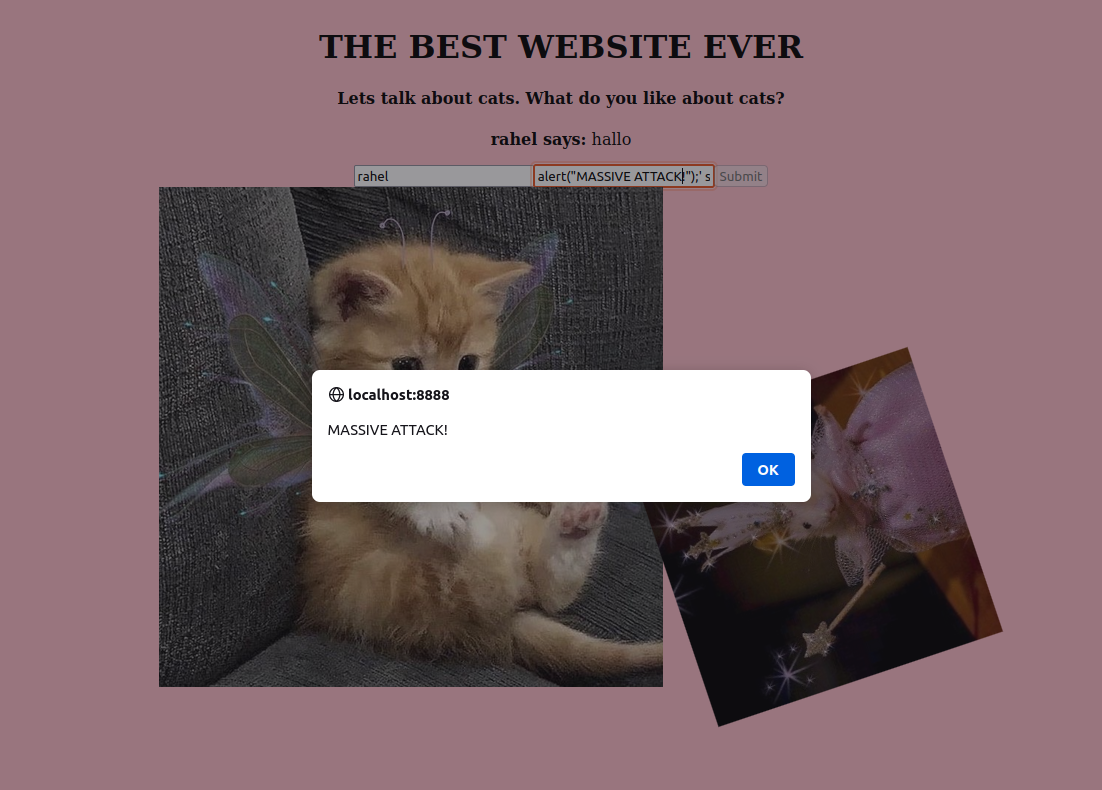
\includegraphics[width=0.8\textwidth,height=\textheight,keepaspectratio]{07_css.png}
\end{frame}

\begin{frame}[c]{Features}
   \begin{itemize}
       \item Multiple Users can connect concurrently 
       \item Error handling 
       \item Process HTTP Requests (GET, POST, HEAD)
       \item CGI (Common Gateway Interface) Support
       \item Log web traffic 
       \item Multiple domain support
       \item User Configuration
       \item Containerization
   \end{itemize} 
\end{frame}

\begin{frame}[c]{Configuration: Multi domain support}
    \centering
    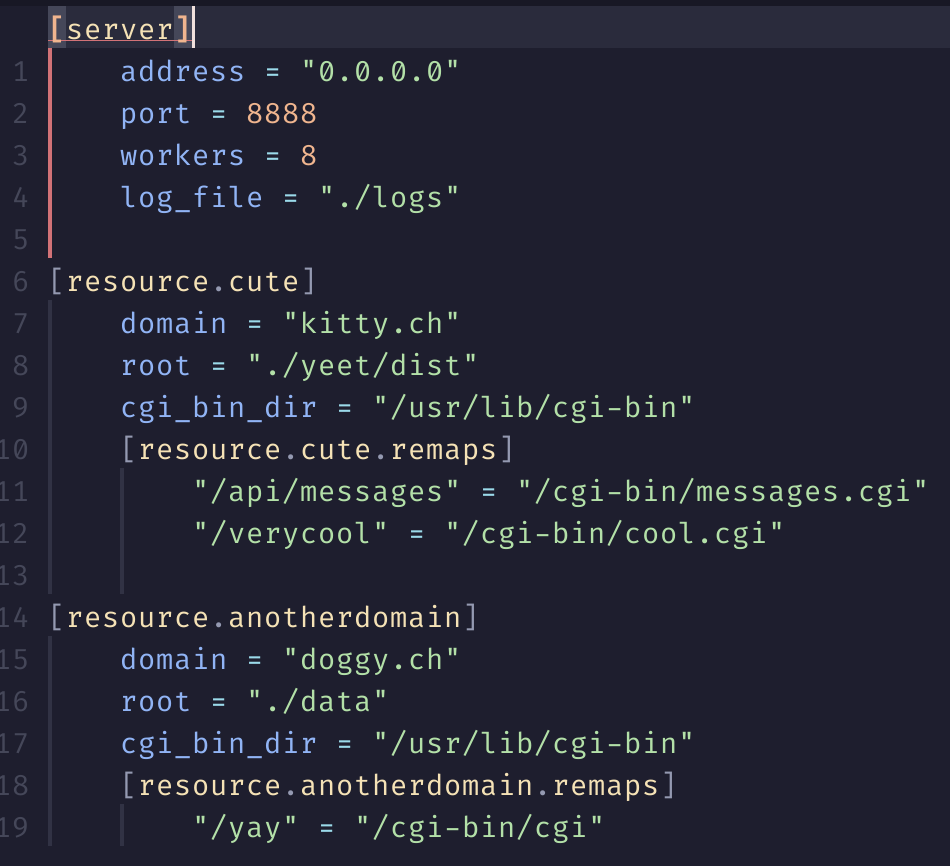
\includegraphics[width=0.8\textwidth,height=0.8\textheight,keepaspectratio]{config.png}
\end{frame}

\begin{frame}[c]{Implementation: Conceptual Overview}
    \centering
    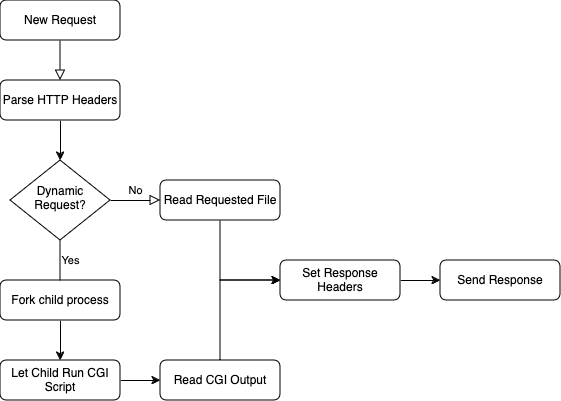
\includegraphics[width=0.8\textwidth,height=0.8\textheight,keepaspectratio]{web_server_inner_workings.png}
\end{frame}

\begin{frame}[c]{Libraries}
    \centering
    \begin{itemize}
        \item Hashmap %\url{https://github.com/tezc/sc}
        \item Logging %\url{https://github.com/rxi/log.c}
        \item Threadpool %\url{https://github.com/Pithikos/C-Thread-Pool}
        \item TOML Parser %\url{https://github.com/cktan/tomlc99}
    \end{itemize}
\end{frame}

\begin{frame}[c]{Demo}
    \centering
    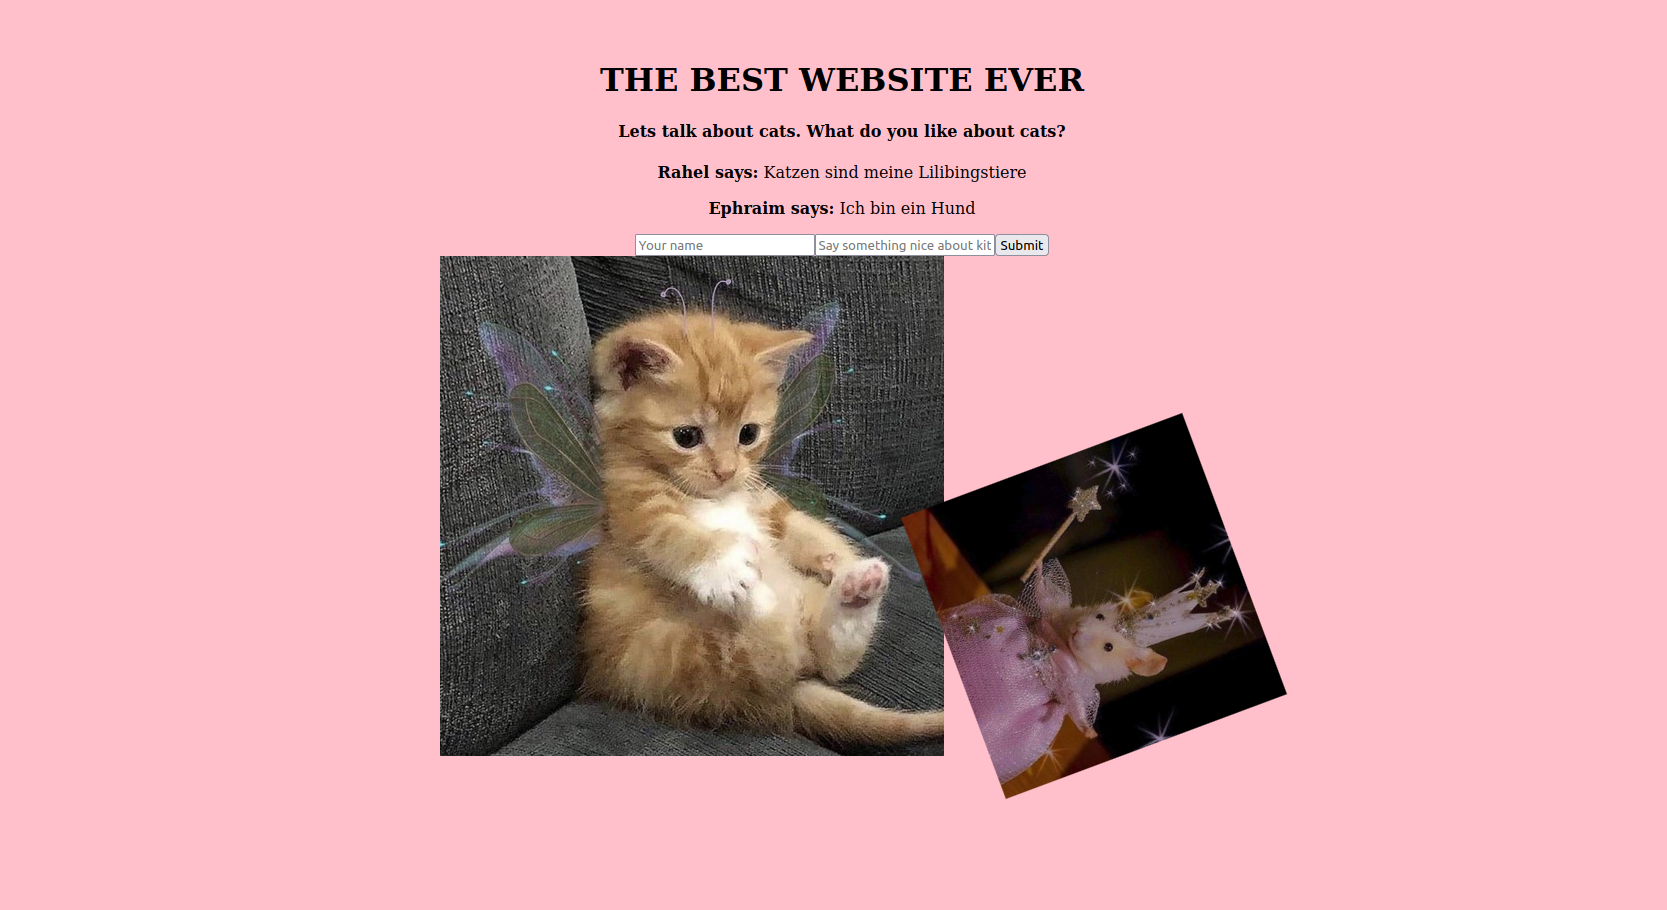
\includegraphics[width=0.8\textwidth,height=0.8\textheight,keepaspectratio]{demo.png}
\end{frame}

\begin{frame}[c]{Lessons Learned}
    \centering
    \begin{itemize}
        \item OS Knowledge 
        \item C Programming 
        \item Reproducibility
    \end{itemize}
\end{frame}

\begin{frame}[c]{Conclusion}
    \begin{itemize}
        \item Didn't look at the time plan, but we are very efficient spontaneous workers 
        \item From the initial project plan we implemented everything but Websockets. 
        \item Overall we are very happy with our results :)
    \end{itemize}
    \vspace{\baselineskip}
    \textbf{Future Outlook}: \\ 
    \begin{itemize}
        \item Websockets 
        \item Security 
        \item fastCGI 
    \end{itemize}
\end{frame}

\begin{frame}[t,plain]
  \lastpage{{\usebeamerfont{title} Questions?}}
\end{frame}

\end{document}

